\let\negthickspace\undefined
\documentclass[journal,12pt,twocolumn]{IEEEtran}
\usepackage{cite}
\usepackage{amsmath,amssymb,amsfonts,amsthm}
\usepackage{algorithmic}
\usepackage{graphicx}
\usepackage{textcomp}
\usepackage{xcolor}
\usepackage{txfonts}
\usepackage{listings}
\usepackage{enumitem}
\usepackage{mathtools}
\usepackage{gensymb}
\usepackage{comment}
\usepackage[breaklinks=true]{hyperref}
\usepackage{tkz-euclide} 
\usepackage{listings}
\usepackage{gvv}                                        
\def\inputGnumericTable{}                                 
\usepackage[latin1]{inputenc}                                
\usepackage{color}                                            
\usepackage{array}                                            
\usepackage{longtable}                                       
\usepackage{calc}                                             
\usepackage{multirow}                                         
\usepackage{hhline}                                           
\usepackage{ifthen}                                           
\usepackage{lscape}
\setlength{\arrayrulewidth}{0.5mm}
\setlength{\tabcolsep}{18pt}
\renewcommand{\arraystretch}{1.5}
\newtheorem{theorem}{Theorem}[section]
\newtheorem{problem}{Problem}
\newtheorem{proposition}{Proposition}[section]
\newtheorem{lemma}{Lemma}[section]
\newtheorem{corollary}[theorem]{Corollary}
\newtheorem{example}{Example}[section]
\newtheorem{definition}[problem]{Definition}
\newcommand{\BEQA}{\begin{eqnarray}}
\newcommand{\EEQA}{\end{eqnarray}}
\newcommand{\define}{\stackrel{\triangle}{=}}
\theoremstyle{remark}
\newtheorem{rem}{Remark}
\begin{document}
\title{Sequence(19) 10.5.3}
\author{EE23BTECH11051-Rajnil Malviya}
\date{January 2024}
\maketitle
\subsection*{\textit{Question :-}}
200 logs are stacked in the following manner: 20 logs in the bottom row, 19 in the next row,
18 in the row next to it and so on . In how many rows are the 200 logs placed
and how many logs are in the top row?
\begin{table}[h!]
   
        \begin{tabular}{ | m{1.0cm} | m{4cm} | } 
  \hline
 Symbol & Description \\ 
 \hline
 $n$ & term number \\
 \hline
$x(n)$ & $n_{th}$ term of A.P\\ 
\hline
 d & common difference of A.P \\
\hline
$S_n $& Sum upto $n_{th}$ of A.P \\
\hline

\end{tabular}\\
\caption{}
\label{Table:1}
       
    \end{table}


For an Arithmetic Progression :-
\begin{align}x(n)-x(n-1) \; = \; d \end{align}
\begin{align}x(n-1)-x(n-2) \; = \; d \end{align}
\begin{align}x(n-2)-x(n-3) \; = \; d \end{align}
$$.$$
$$.$$
$$.$$
\begin{align}x(2)-x(1) \; = \; d \end{align}
adding all these equations :-
\begin{align}x(n)-x(1) \; = \; \brak{n-1} d \end{align}
\begin{align}x(n) \; = \; x(1)+\brak{n-1} d \end{align}
Sum upto n terms of A.P :-
\begin{align}S_n=x(1)+x(2)+....+x(n)\end{align}
\begin{align}S_n=x(n)+x(n-1)+....+x(1)\end{align}
adding equations 7 and 8 \\
$2 S_n=[x(1)+x(n))+(x(2)+x(n-2))+...$\\\begin{align}...+(x(n)+x(1)]\end{align}
Substituting by using equation 6 \\
$2 S_n=[x(1)+(x(1) +(n-1) d)]+ ...$
\begin{align}....+[(x(1) + (n-1) d) + x(1)]\end{align}
\begin{align}S_n=\frac{n}{2}\brak{2x(1) + (n-1) d}\end{align}
\subsection*{\textit{Solution :-}}
\begin{table}[h!]
   
        \begin{tabular}{ | m{1.0cm} | m{4cm} | } 
  \hline
 Symbol & Value \\ 
 \hline
$x(1)$& 20 (logs in bottom row) \\
\hline
$x(2)$ & 19\\ 
\hline
$x(3)$ & 18\\ 
\hline
$S_n$& 200 (total number of logs) \\
\hline
\end{tabular}\\
\caption{}
\label{Table:1}
       
    \end{table}
Using equation 4 


\begin{align}d=x(2)-x(1)\end{align}
Using equation 6
\begin{align}x(n) &= \brak{21-n}\end{align}
\subsection*{\textit{Z Transformation :-}}
The relation between \(x(n)\) and \(u(n)\):
\begin{align}
 x(n) &= \brak{21-n} u(n)\label{eq:1}
\end{align}
\begin{align}
   u(n) &\overset{\text{ZT}}{\longleftrightarrow} \frac{1}{(1 - z^{-1})}
    \text{ [ROC: } \lvert z \rvert > 1\text{]}\end{align} \\
  \begin{align}  U(z)=\frac{1}{(1 - z^{-1})}\end{align}
Z-transform of \(n^ku(k)\) in terms of the \(k\)-th derivative of \(U(z)\):

\begin{align}
n^k u(n) &\overset{\text{ZT}}{\longleftrightarrow} (-1)^k z^k \frac{d^k}{dz^k}U(z)
\end{align}
\begin{align}
    nu(n) &\system{Z} \frac{z^{-1}}{(1 - z^{-1})^2} \quad \abs{ z} > 1  \label{eq:3} \\
    n^2u(n) &\system{Z} \frac{(z^{-1})(1+z^{-1})}{(1 - z^{-1})^3} \quad \abs{ z} > 1  \label{eq:4} \\
    n^3u(n) &\system{Z} \frac{(z^{-1})(1+4z^{-1}+z^{-2})}{(1 - z^{-1})^4} \quad \abs{ z} > 1  \label{eq:5} 
\end{align}
Referencing the equations from 14,18,19
\begin{align}
    x(n) &\system{Z} \frac{21}{(1 - z^{-1})} +\frac{(z^{-1})(1+z^{-1})}{(1 - z^{-1})^3} \quad \abs{ z} > 1  \label{eq:3} 
\end{align}
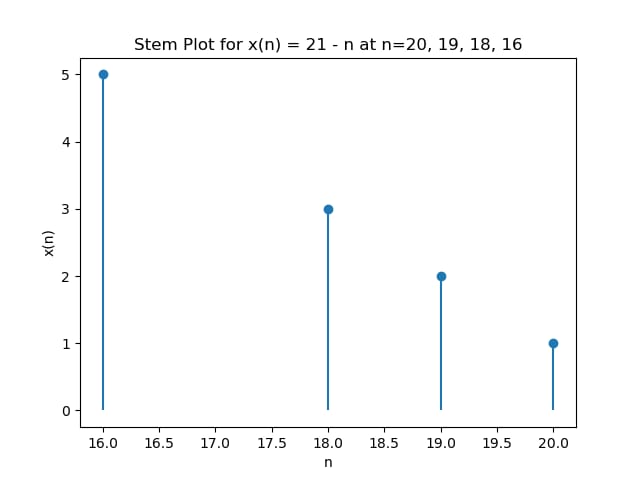
\includegraphics[width=1\linewidth]{figs/f1.jpeg}\\\\
Substituting from Table:II
\begin{align}d=-1\end{align}
\begin{table}[h!]
        \begin{tabular}{ | m{1.0cm} | m{4cm} | } 
  \hline
 Symbol & Description \\ 
 
 \hline

$x(n)$ & number of logs in top most row \\ 
\hline
\end{tabular}\\
\caption{}
\label{Table:1}
    \end{table}
For Practical reasons 
\begin{align}x(n)>0\end{align}
Using equation 13 and substituting in equation 6
\begin{align}20+(n-1)(-1)>0\end{align}
\begin{align}n<21\end{align}
Using equation 11 and substituting from Table:2
\begin{align}n^2-41 n +400 = 0\end{align}
\begin{align}n=16\; ,\;25\end{align}
From equation 16 
\begin{align}n=16\end{align}
Substituting in equation 6
\begin{align}x(n)=20+(16-1)(-1)\end{align}
\begin{align}a_n=5\end{align}
Ans . There are 16 rows and 5 logs in top row 
\end{document}
